\section{Billboard-based visualization}
In this section we present the work of Ohta et al. \cite{billboard}.
The authors use billboard representation to make a 3D model of each player.
This method is simpler than full 3D reconstruction and require less computation.
A player billboard is a small rectangle standing perpendicular to the ground
and a 2D texture is shown on it.
The difference between 3D reconstruction and billboard representation is shown in Figure \ref{fig:billboard_comparison}:
the visual difference is clear at a close viewpoint but becomes very small at a distant viewpoint.

\begin{figure}[htbp]
\centerline{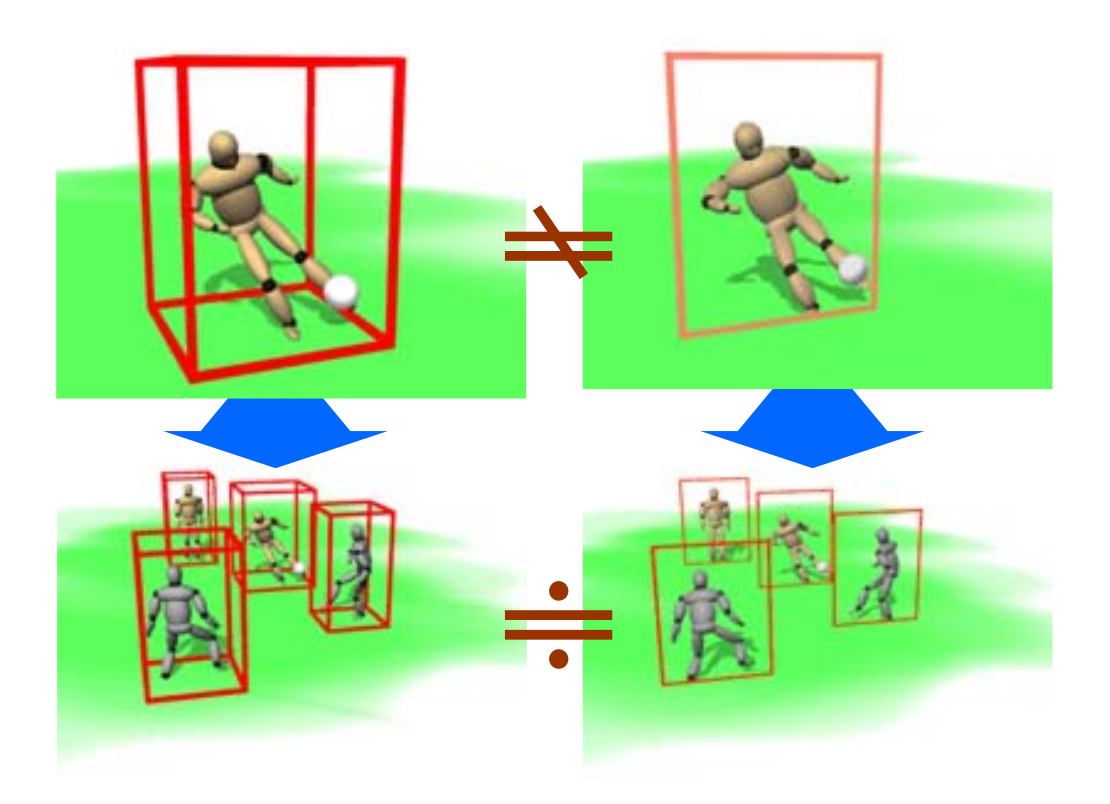
\includegraphics[scale=0.22]{billboard_comparison.png}}
\caption{Appearance similarity between 3D reconstruction and billboard in close and distant view \cite{billboard}}
\label{fig:billboard_comparison}
\end{figure}